\chapter{Sensors}
\label{chapter:Sensors}

In this chapter will is briefly explained several notations used along the report and
important definitions that help the reader to walk through the work. Many parts of the text presented here are extracted from \cite{thesis_BT} where full description is available and user should refer to it, if necessary. 
The notation system of leading superscripts and subscripts is used to denote
relative frames orientation or general physical quantities (vectors, points).
For frames orientations, leading subscript refers to the frame being represented
with respect to the frame in leading superscript. For example let R be a
rotation matrix. Using the notations stated before, ${}^a_bR$ describes
orientation of frame $b$ with respect to frame $a$. For physical quantities, a
vector is represented in the frame defined by is leading superscript,
${}^av$ and in similar way points follow the same rule,
${}^aP=[{}^ax,{}^ay,{}^az]$.


\section{Definition of frames} \label{section:frames}

The frames cited are \gls{ECEF}, \gls{WGS84},
\gls{ENU} and body frame. The \gls{ECEF}, \gls{WGS84} are just auxiliary frames
used to define the \gls{ENU} frame which will be considered the world frame.


\subsection{ECEF and ENU Frame}

\gls{ECEF} coordinate system defines a referential axis where the origin is
defined as the center of Earth, X axis is defined through the intersection of
the plan defined by zero latitude line (Equator) and plan defined by zero
longitude line (prime meridian). The X-axis orientation is considered positive
from center towards the point defined by zero latitude and zero longitude. Z axis
is defined by line intersecting origin and both Poles, being positive towards
North Pole. Y axis is perpendicular to the plan defined by X and Z axis and it
positive direction is defined by right hand rule.

\begin{figure}[!htb]
	\centering
	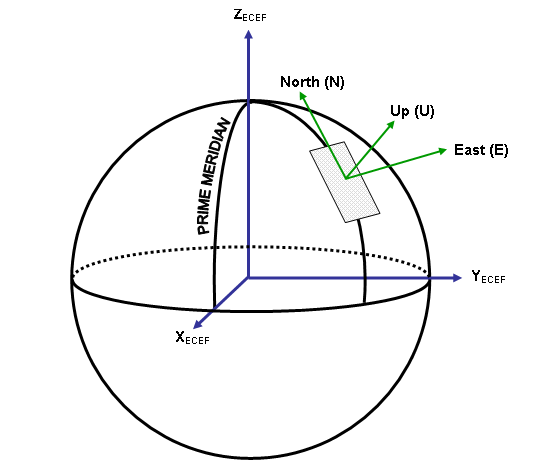
\includegraphics[width=0.3\linewidth]{figures/EarthTangentialPlane.png}
	\caption[ECEF frame and Local ENU frame.]{ECEF frame and Local ENU frame (\href{https://en.wikipedia.org/wiki/File:EarthTangentialPlane.png}{source:wikipedia})}. 
	\label{fig:ecef_enu} 
\end{figure}

\gls{ENU} coordinate system is a local coordinate system where the origin is
located at a user defined point in \gls{ECEF} coordinate system, with Y axis pointing
towards North Pole and X axis pointing towards East. The plan defined by X and Y
axis is tangent to the \gls{WGS84} frame on the origin of ENU. Z axis express
the altitude from defined local plane (see figure \ref{fig:ecef_enu}). The
\gls{ENU} frame is considered in this work as the reference frame and will be
denoted with superscript or subscript $w$.

Given a point of reference in \gls{ECEF} frame, it is necessary to find the
corresponding latitude and longitude of reference point ($X_r,Y_r,Z_r$). To do
it is necessary to use the parameters of \gls{WGS84} presented in the table
\ref{tab:wgs84_parameters}

\begin{table}[!htb]
	\centering
	\begin{tabular}{lll}
		\toprule
		\multicolumn{3}{c}{\textbf{WGS 84 Defining Parameters}\cite{wgs84_params}}\\
		\midrule
		\textbf{Parameter}        & \textbf{Notation} & \textbf{Value} \\
		\midrule
		Semi-major axis           & $a$   & 6 378 137.0 m   \\
		Reciprocal of flattening  & $1/f$ & 298.257 223 563 \\
		Semi-minor axis 		  & $b$   & 6 356 752.3142 m\\
		First eccentricity squared& $e^2$ & 6.694 379 990 14x10\textsuperscript{-3}\\
		Second eccentricity squared &${e'}^2$ &  6.739 496 742 28x10\textsuperscript{-3}\\
		\bottomrule
	\end{tabular}
	\caption[WGS84 parameters necessary to transform ECEF coordinates into ENU]{WGS84 parameters necessary to transform ECEF coordinates into ENU}
	\label{tab:wgs84_parameters}
\end{table}

Using set of equations \eqref{eq:ecef_enu_auxiliary} to estimate the latitude
($\lambda_r$) and longitude ($\varphi_r$) for the reference coordinate point.
The final transformation results in applying \eqref{eq:ecef_enu} to
\gls{ECEF} physical quantities \cite{ecef_enu}.

\begin{subequations}
	\label{eq:ecef_enu_auxiliary}
	\begin{equation}
	p = \sqrt{{X_r}^2 + {Y_r}^2}
	\end{equation}
	\begin{equation}
	\theta = \arctan\bigg(Z_r\frac{a}{pb}\bigg)
	\end{equation}
	\begin{equation}
	\lambda_r = \arctantwo(Y_r,X_r)
	\end{equation}
	\begin{equation}
	\varphi_r = \arctan\bigg(\frac{Z_r + e^2b\sin^3(\theta)}{p-{e'}^2a\cos^3(\theta)}\bigg)
	\end{equation}
\end{subequations}

\begin{equation}
\begin{bmatrix}
X\\
Y\\
Z
\end{bmatrix}_{ENU} =
\begin{bmatrix}
-\sin(\lambda_r)   				& \cos(\varphi_r) 				  & 0               \\
-\sin(\varphi_r)\cos(\lambda_r) & -\sin(\varphi_r)\sin(\lambda_r) & \cos(\varphi_r) \\
\cos(\varphi_r)\cos(\lambda_r)  & \cos(\varphi_r)\sin(\lambda_r)  & \sin(\varphi_r)  
\end{bmatrix}
\begin{bmatrix}
X-X_r\\
Y-Y_r\\
Z-Z_r
\end{bmatrix}_{ECEF}
\label{eq:ecef_enu}
\end{equation}

\subsection{Body frame, \textit{b}}\label{subsection:body_frame}

Each sensor present in the razor board is aligned to match the sensor axes
printed in the board as seen in figure \ref{fig:razor9dof}. For simplicity, the
razor sensor is placed as possible near the middle point of the bisector
segment between the two wheel axes in such a away that YY axis as marked in the
figure \ref{fig:razor9dof} is pointing towards the front of vehicle, XX axis is
pointing to the right side of the car and ZZ axis is pointing to the top. This
way, if the Euler angles describing the orientation of body frame related to
world frame are all equal to zero, it means the axes in each frame are
coincident apart from an offset in origin.
Rotation angles are considered positive following the right hand rule in each axis.
The origin of body frame is equal to intersection of rear wheel axis with the bisector defined above.

\section{Euler angles and Rotation Matrix} \label{section:euler_matrix_def}

\begin{figure}[hb]
	\centering
	\subcaptionbox{3D view of axes frames example\label{subcap:3D_view_axis_example}}{
		\tdplotsetmaincoords{45}{70}
		\begin{tikzpicture}[scale=3, tdplot_main_coords]
		
		%draw a grid in the x-y plane
		\foreach \xgrid in {-1,-0.9,...,1.1}
		\foreach \ygrid in {-1,-0.9,...,1.1}
		{
			\draw[very thin,gray!30] (\xgrid,-1) -- (\xgrid,1);
			\draw[very thin,gray!30] (-1,\ygrid) -- (1,\ygrid);
		}
		
		%---------------------------------------------------------------------------------
		% Extend axis backwards
		%---------------------------------------------------------------------------------
		\draw[dashed] (0,0,0) -- ( -1, 0, 0);
		\draw[dashed] (0,0,0) -- (  0, -1, 0);
		%\draw[dashed] (0,0,0) -- ( 0, 0, -1);
		
		%---------------------------------------------------------------------------------
		% Plot new frame axis
		%---------------------------------------------------------------------------------
		\draw[->, bluemat] (0,0,0) -- ( 0.5000,  0.5000, 0.7071) node[anchor=south]{${}^bx$};
		\draw[->, redmat](0,0,0) -- (-0.8536,  0.1464, 0.5000) node[anchor=south]{${}^by$};
		\draw[->, yellowmat]  (0,0,0) -- ( 0.1464, -0.8536, 0.5000) node[anchor=south]{${}^bz$};
		
		%---------------------------------------------------------------------------------
		% guides for XX axis
		%---------------------------------------------------------------------------------
		% dashed lines x
		\draw[dashed, bluemat] (0.5000, 0, 0) -- ( 0.5000, 0.5000, 0) node[pos=0.5, anchor=north]{\small $r_{xy}$};
		% dashed lines y
		\draw[dashed, bluemat] ( 0, 0.5000, 0) -- ( 0.5000, 0.5000, 0) node[pos=0.5, rotate=-60, anchor=north]{\small $r_{xx}$};
		% dashed lines z
		\draw[dashed, bluemat] ( 0.5000, 0.5000, 0) -- ( 0.5000,  0.5000, 0.7071) node[pos=0.5, rotate=90, anchor=north]{\small $r_{xz}$};
		%---------------------------------------------------------------------------------
		% guides for YY axis
		%---------------------------------------------------------------------------------
		% dashed lines x
		\draw[dashed, redmat] (-0.8536, 0, 0) -- (-0.8536, 0.1464, 0) node[pos=0.5,anchor=north]{\small $r_{yy}$};
		% dashed lines y
		\draw[dashed, redmat] (0, 0.1464, 0) -- (-0.8536, 0.1464, 0) node[pos=0.5, rotate=-60, anchor=south]{\small $r_{yx}$};
		% dashed lines z
		\draw[dashed, redmat] (-0.8536, 0.1464, 0) -- (-0.8536,  0.1464, 0.5000) node[pos=0.5,rotate=90,anchor=south]{\small $r_{yz}$};
		%---------------------------------------------------------------------------------
		% guides for ZZ axis
		%---------------------------------------------------------------------------------
		% dashed lines x
		\draw[dashed, yellowmat] (0, -0.8536, 0) -- ( 0.1464, -0.8536, 0) node[pos=0.5,anchor=east]{\small $r_{zx}$};
		% dashed lines y
		\draw[dashed, yellowmat] (0.1464, 0, 0) -- ( 0.1464, -0.8536, 0) node[pos=0.5,anchor=north]{\small $r_{zy}$};
		% dashed lines z
		\draw[dashed, yellowmat] ( 0.1464, -0.8536, 0) -- ( 0.1464, -0.8536, 0.5000) node[pos=0.5,rotate=90,anchor=north]{\small $r_{zz}$};
		
		% Draw main coordinate system
		\draw[thick,->] (0,0,0) -- (1,0,0) node[anchor=north east]{${}^ax$};
		\draw[thick,->] (0,0,0) -- (0,1,0) node[anchor=north west]{${}^ay$};
		\draw[thick,->] (0,0,0) -- (0,0,1) node[anchor=south]{${}^az$};
		
		\end{tikzpicture}}
	\hfill
	\subcaptionbox{XY plane of axes frame example\label{subcap:axis_example_xy_plane}}{
		\tdplotsetmaincoords{0}{0}
		\begin{tikzpicture}[scale=3, tdplot_main_coords]
		
		%draw a grid in the x-y plane
		\foreach \xgrid in {-1,-0.9,...,1.1}
		\foreach \ygrid in {-1,-0.9,...,1.1}
		{
			\draw[very thin,gray!30] (\xgrid,-1) -- (\xgrid,1);
			\draw[very thin,gray!30] (-1,\ygrid) -- (1,\ygrid);
		}
		
		%---------------------------------------------------------------------------------
		% Extend axis backwards
		%---------------------------------------------------------------------------------
		\draw[dashed] (0,0,0) -- ( -1, 0, 0);
		\draw[dashed] (0,0,0) -- (  0, -1, 0);
		%\draw[dashed] (0,0,0) -- ( 0, 0, -1);
		
		%---------------------------------------------------------------------------------
		% Plot new frame axis
		%---------------------------------------------------------------------------------
		\draw[->, bluemat] (0,0,0) -- ( 0.5000,  0.5000, 0.7071) node[anchor=south]{${}^bx$};
		\draw[->, redmat](0,0,0) -- (-0.8536,  0.1464, 0.5000) node[anchor=south]{${}^by$};
		\draw[->, yellowmat]  (0,0,0) -- ( 0.1464, -0.8536, 0.5000) node[anchor=west]{${}^bz$};
		
		%---------------------------------------------------------------------------------
		% guides for XX axis
		%---------------------------------------------------------------------------------
		% dashed lines x
		\draw[dashed, bluemat] (0.5000, 0, 0) -- ( 0.5000, 0.5000, 0) node[pos=0.5, anchor=west]{\small $r_{xy}$};
		% dashed lines y
		\draw[dashed, bluemat] ( 0, 0.5000, 0) -- ( 0.5000, 0.5000, 0) node[pos=0.5, anchor=south]{\small $r_{xx}$};
		% dashed lines z
		%\draw[dashed, bluemat] ( 0.5000, 0.5000, 0) -- ( 0.5000,  0.5000, 0.7071) node[pos=0.5, rotate=90, anchor=north]{\small $r_{xz}$};
		%---------------------------------------------------------------------------------
		% guides for YY axis
		%---------------------------------------------------------------------------------
		% dashed lines x
		\draw[dashed, redmat] (-0.8536, 0, 0) -- (-0.8536, 0.1464, 0) node[pos=0.5,anchor=east]{\small $r_{yy}$};
		% dashed lines y
		\draw[dashed, redmat] (0, 0.1464, 0) -- (-0.8536, 0.1464, 0) node[pos=0.5, anchor=south]{\small $r_{yx}$};
		% dashed lines z
		%\draw[dashed, redmat] (-0.8536, 0.1464, 0) -- (-0.8536,  0.1464, 0.5000) node[pos=0.5,rotate=90,anchor=south]{\small $r_{yz}$};
		%---------------------------------------------------------------------------------
		% guides for ZZ axis
		%---------------------------------------------------------------------------------
		% dashed lines x
		\draw[dashed, yellowmat] (0, -0.8536, 0) -- ( 0.1464, -0.8536, 0) node[pos=0.5,anchor=north]{\small $r_{zx}$};
		% dashed lines y
		\draw[dashed, yellowmat] (0.1464, 0, 0) -- ( 0.1464, -0.8536, 0) node[pos=0.5,anchor=west]{\small $r_{zy}$};
		% dashed lines z
		%\draw[dashed, yellowmat] ( 0.1464, -0.8536, 0) -- ( 0.1464, -0.8536, 0.5000) node[pos=0.5,rotate=90,anchor=north]{\small $r_{zz}$};
		
		% Draw main coordinate system
		\draw[thick,->] (0,0,0) -- (1,0,0) node[anchor=north east]{${}^ax$};
		\draw[thick,->] (0,0,0) -- (0,1,0) node[anchor=north west]{${}^ay$};
		%\draw[thick,->] (0,0,0) -- (0,0,1) node[anchor=south]{${}^az$};
		
		\end{tikzpicture}
		
	}
	\caption[Two frames axes example]{Two frames axes example}
	\label{fig:frame_axis_example}
\end{figure}


The rotation matrix is a tool used to describe transformation of coordinates
from one frame to another and this also describe orientation of one frame
relative to another frame. The convention used in this work is represented by \eqref{eq:rotation_matrix} and maps quantities described in frame $b$ to
frame $a$. Comparing the structure of \eqref{eq:rotation_matrix} with
figure \ref{fig:frame_axis_example} it is seen that columns of ${}^a_bR$
represent each unity vector defining all axes of frame $b$.



\begin{equation}
{}^a_bR=\begin{bmatrix}
{}^ar_{xx} & {}^ar_{yx} & {}^ar_{zx}\\
{}^ar_{xy} & {}^ar_{yy} & {}^ar_{zy}\\
{}^ar_{xz} & {}^ar_{yz} & {}^ar_{zz}
\end{bmatrix}
\label{eq:rotation_matrix}
\end{equation}

Rotation matrices belong to the orthonormal group and one important property
is that ${}^a_bR{}^a_bR^T=I$ meaning ${}^a_bR^T = {}^a_bR^{-1}$. Also
${}^a_bR^T$ is equal to ${}^b_aR$
\cite{Sequeira2016}\cite{wiki_rotationtheorem}.


Euler angles are another form to describe orientation of one frame relative to
another by defining three angles. The Euler angles convention adopted in this
work is the Tait–Bryan \gls{intrinsic} rotation sequence Z-Y-X, meaning
referential $a$ axes, represented in figure \ref{fig:frame_axis_example}, can be
mapped into referential $b$ by performing sequential rotations, first along ZZ
axis by an angle $\psi$, second along the resulting YY axis by an angle $\theta$
and final rotation along the resulting XX axis by an angle $\phi$. In figure
\ref{fig:frame_axis_example_euler} is represented the sequence necessary to
rotate frame $a$ into frame $b$ with the respective Euler angles to achieve the
same orientation as expressed in figure \ref{fig:frame_axis_example}. It is also
represented the intermediary axes resulting from each sequential rotation and it
positive direction. Each individual rotation is expressed by is own rotation
matrix using the respective Euler angle associated and the final orientation is
the result of successive matrices multiplications as shown in equation
\ref{eq:rotMat_composition} where the intermediary axes sequence is denoted as
expressed in the figure \ref{fig:frame_axis_example_euler}.

\begin{equation}
\begin{aligned}
{}^b_aR&={}^b_2R_x(\phi){}^2_1R_y(\theta){}^1_aR_z(\psi)\\
&=\begin{bmatrix}
\cos(\psi)\cos(\theta) 								  & \sin(\psi)\cos(\theta) 								  & -\sin(\theta)         \\
\cos(\psi)\sin(\theta)\sin(\phi)-\sin(\psi)\cos(\phi) & \cos(\psi)\cos(\phi)+\sin(\psi)\sin(\theta)\sin(\phi) & \cos(\theta)\sin(\phi)\\
\sin(\psi)sin(\phi)+\cos(\psi)\sin(\theta)\cos(\phi)  & \sin(\psi)\sin(\theta)\cos(\phi)-\cos(\psi)\sin(\phi) & \cos(\theta)\cos(\phi)
\end{bmatrix}
%				  \begin{bmatrix} % the usual transpose
%				  \cos(\psi)\cos(\theta) & \cos(\psi)\sin(\theta)\sin(\phi)-\sin(\psi)\cos(\phi) & \sin(\psi)sin(\phi)+\cos(\psi)\sin(\theta)\sin(\phi)\\
%				  \sin(\psi)\cos(\theta) & \cos(\psi)\cos(\phi)+\sin(\psi)\sin(\theta)\sin(\phi) & \sin(\psi)\sin(\theta)\cos(\phi)-\cos(\psi)\sin(\phi)\\
%				  -\sin(\theta)		   & \cos(\theta)\sin(\phi)								   & \cos(\theta)\cos(\phi)
%				  \end{bmatrix}
\end{aligned}
\label{eq:rotMat_composition}
\end{equation}

\begin{figure}[!hbt]
	\centering
	% Set the plot display orientation
	% Syntax: \tdplotsetdisplay{\theta_d}{\phi_d}
	\tdplotsetmaincoords{75}{120}
	
	\pgfmathsetmacro{\zRot}{45}
	\pgfmathsetmacro{\yRot}{-45}
	\pgfmathsetmacro{\xRot}{45}
	%%%%%% Change the rotation matrix in order to use Tait-Bryan angles
	\tdseteulerxyz
	%%%%%%%%%%%%% Z-Y-X
	\begin{tikzpicture}[scale=4,tdplot_main_coords]
	\foreach \xgrid in {-1,-0.9,...,1.1}
	\foreach \ygrid in {-1,-0.9,...,1.1}
	{
		\draw[very thin,gray!30] (\xgrid,-1) -- (\xgrid,1);
		\draw[very thin,gray!30] (-1,\ygrid) -- (1,\ygrid);
	}
	
	%---------------------------------------------------------------------------------
	% Extend axis backwards
	%---------------------------------------------------------------------------------
	\draw[dashed] (0,0,0) -- ( -1, 0, 0);
	\draw[dashed] (0,0,0) -- (  0, -1, 0);
	%\draw[dashed] (0,0,0) -- ( 0, 0, -1);
	% Set origin of main (body) coordinate system
	\coordinate (O) at (0,0,0);
	
	% Draw main coordinate system
	\draw[thick,->] (0,0,0) -- (1,0,0) node[anchor=north east]{\tiny ${}^ax$};
	\draw[thick,->] (0,0,0) -- (0,1,0) node[anchor=north west]{\tiny ${}^ay$};
	\draw[thick,->] (0,0,0) -- (0,0,1) node[anchor=south]{\tiny ${}^az$};
	
	%Draws arc representing the rotated angle.
	\tdplotdrawarc[thick,tdplot_main_coords,->, color=black]{(0,0,0)}{0.5}{0}{\zRot}{anchor=north,color=black}{\tiny $\psi$}
	%Draws circle representing the rotated planes. Each of these should be "pointed" by two arrows.
	\tdplotdrawarc[dashed,tdplot_main_coords,->, color=black]{(0,0,1)}{0.1}{0}{359}{}{}
	
	
	
	% First intrinsic rotation
	\tdplotsetrotatedcoords{\zRot}{0}{0}
	\draw[thick,tdplot_rotated_coords,->, yellowmat] (0,0,0) -- (0.9,0,0) node[anchor=west]{\tiny ${}^1x$};
	\draw[thick,tdplot_rotated_coords,->, yellowmat] (0,0,0) -- (0,0.9,0) node[anchor=west]{\tiny ${}^1y$};
	\draw[thick,tdplot_rotated_coords,->, yellowmat] (0,0,0) -- (0,0,0.9) node[anchor=north west]{\tiny ${}^1z$};
	
	% make xy plane in vertical to mark angle
	\tdplotsetrotatedcoords{\zRot}{0}{90}
	\tdplotdrawarc[thick,tdplot_rotated_coords,->,color=yellowmat]{(0,0,0)}{0.5}{0}{-\yRot}{anchor=west,color=yellowmat}{$\theta$}
	\tdplotdrawarc[dashed,tdplot_rotated_coords,->,color=yellowmat]{(0,0,-0.9)}{0.1}{0}{-359}{}{}
	%	% auxiliary axis to confirm correct plan
	%	\draw[thick,tdplot_rotated_coords,->] (0,0,0) -- (1,0,0) node[anchor=north east]{${}^tx$};
	%	\draw[thick,tdplot_rotated_coords,->] (0,0,0) -- (0,1,0) node[anchor=north west]{${}^ty$};
	%	\draw[thick,tdplot_rotated_coords,->] (0,0,0) -- (0,0,1) node[anchor=south]{${}^tz$};
	
	% second intrinsic rotation
	\tdplotsetrotatedcoords{\zRot}{\yRot}{0}
	\draw[thick,tdplot_rotated_coords,->, redmat] (0,0,0) -- (0.8,0,0) node[anchor=west]{\tiny ${}^2x$};
	\draw[thick,tdplot_rotated_coords,->, redmat] (0,0,0) -- (0,0.8,0) node[anchor=north]{\tiny ${}^2y$};
	\draw[thick,tdplot_rotated_coords,->, redmat] (0,0,0) -- (0,0,0.8) node[anchor=south]{\tiny ${}^2z$};
	
	% make xy plan in vertical to mark angle b
	\tdplotsetrotatedcoords{90+\zRot}{0}{\xRot}
	\tdplotdrawarc[thick,tdplot_rotated_coords,->,color=redmat]{(0,0,0)}{0.5}{0}{\xRot}{anchor=west,color=redmat}{$\phi$}
	\tdplotdrawarc[dashed,tdplot_rotated_coords,->,color=redmat]{(0,0,0.8)}{0.1}{0}{359}{}{}
	%	% auxiliary axis to confirm correct plan
	%	\draw[thick,tdplot_rotated_coords,->] (0,0,0) -- (1,0,0) node[anchor=north east]{${}^tx$};
	%	\draw[thick,tdplot_rotated_coords,->] (0,0,0) -- (0,1,0) node[anchor=north west]{${}^ty$};
	%	\draw[thick,tdplot_rotated_coords,->] (0,0,0) -- (0,0,1) node[anchor=south]{${}^tz$};
	
	% second intrinsic rotation
	\tdplotsetrotatedcoords{\zRot}{\yRot}{\xRot}
	\draw[thick,tdplot_rotated_coords,->, bluemat] (0,0,0) -- (1,0,0) node[anchor=west]{\tiny ${}^bx$};
	\draw[thick,tdplot_rotated_coords,->, bluemat] (0,0,0) -- (0,1,0) node[anchor=west]{\tiny ${}^by$};
	\draw[thick,tdplot_rotated_coords,->, bluemat] (0,0,0) -- (0,0,1) node[anchor=south]{\tiny ${}^bz$};
	
	\end{tikzpicture}
	\caption[Two frames axes example - Euler angles]{Two frames axes example - Euler angles. In this case, the angles are $\psi=45^o, \theta=-45^o, \phi=45^o$}
	\label{fig:frame_axis_example_euler}
\end{figure}

\section{Quaternion} \label{section:quaternion}

During the work an \gls{AHRS} algorithm based on \cite{Madgwick2010_report} and derived in \cite{thesis_BT} is implemented  and it uses quaternions. Basic definitions for understanding the filter terminology  are explained in this section following the same notation as present by \cite{thesis_BT} in case the user as no notion of quaternions at all.

Quaternion is a complex number in four dimension that can be used, similar to rotation matrices and Euler angles, to represent orientation of frames with respect to others. The Euler rotation theorem and the Rodriguez formula are the basis for quaternion representation of rotations but will not be discussed. The theorem states it is possible to describe an orientation of frame relative to other by performing a rotation of $\alpha$ along an axis $r$ that is defined by the points that remain static relative to the original frame. \cite{quaternions} quickly resumes the main idea about quaternions, why they can be used to express orientations and relation between them and Euler and Rodriguez formulations. 

A quaternion can be represented by \eqref{eq:quaternion_definition} where $q_1$ is the norm of it, $q_2, q_3$ and $q_4$ are complex coordinates with \textit{i, j, k} being the axis versors. If a quaternion is normalized, it is denoted with a circumflex accent as shown in \eqref{eq:quaternion_normalized}.

\begin{equation}
\centering
\begin{aligned}
q &=q_1+q_2i+q_3j+q_4k\\
q &= [q_1\, q_2\, q_3\, q_4]
\end{aligned}
\label{eq:quaternion_definition}
\end{equation}

\begin{equation}
\centering
\hat{q} \implies \|q\|=1
\label{eq:quaternion_normalized}
\end{equation}

Using the same notation as stated before, ${}^w_bq$ represent the orientation of body frame with respect to world frame. With \eqref{eq:quaternion_definition} in mind, the following list of properties/operations are summarized in this \hyperref[list:quaternion_operations]{list}:

\begin{description}[]
	\label{list:quaternion_operations}
	\item [Identities] All quaternions multiplications must obey to the following set of properties described in equation \ref{eq:quaternion_identities}.
	\begin{subequations}
		\label{eq:quaternion_identities}
		\begin{equation}
		i^2=j^2 = k^2 = ijk = -1
		\end{equation}
		\begin{equation}
		ij =-ji=k
		\end{equation}
		\begin{equation}
		jk =-kj=i
		\end{equation}
		\begin{equation}
		ki =-ik= j
		\end{equation}
	\end{subequations}
	\item [Quaternion multiplication] The quaternions multiplication, denoted by $\otimes$, is defined by the Hamilton product as in equation \ref{eq:quaternion_product}
	\begin{equation}
	\begin{aligned}
	a \otimes b &= [a_1\, a_2\, a_3\, a_4] \otimes [b_1\, b_2\, b_3\, b_4]\\
	&= \begin{bmatrix}
	a_1b_1 -a_2b_2 -a_3b_3 -a_4b_4\\
	a_1b_2 +a_2b_1 +a_3b_4 -a_4b_3\\
	a_1b_3 -a_2b_4 +a_3b_1 +a_4b_2\\
	a_1b_4 +a_2b_3 -a_3b_2 +a_4b_1
	
	\end{bmatrix}^T
	\end{aligned}
	\label{eq:quaternion_product} 
	\end{equation}
	\item [Quaternion conjugate] The quaternion conjugate describes the inverse rotation and is defined as equation \ref{eq:quaternion_conjugate}.
	\begin{equation}
	{}^w_bq^* = {}^b_wq = [q_1\, -q_2\, -q_3\, -q_4]
	\label{eq:quaternion_conjugate} 
	\end{equation}
	\item [Vector rotation] Let's define the following quaternion representation of the same vector but in each referential by using is \gls{pure quaternion} as ${}^wv = [0\,{}^wx\,{}^wy\,{}^wz]$ and ${}^bv = [0\,{}^bx\,{}^by\,{}^bz]$. The rotation of vector $v$ from one frame to other, using a quaternion, is performed by equation \ref{eq:quaternion_rotation}.
	\begin{equation}
	{}^bv = {}^w_b\hat{q} \otimes {}^wv \otimes {}^w_b\hat{q}^*
	\label{eq:quaternion_rotation}
	\end{equation}
	
	\item [Composed rotations] The composition of rotations can be described in quaternions as the product between quaternions. For example the sequence ${}^a_b\hat{q} \rightarrow {}^b_c\hat{q}$ is equal to ${}^a_c\hat{q}$ and is defined as equation \ref{eq:quaternion_composed_rotation}.
	\begin{equation}
	{}^a_c\hat{q} = {}^b_c\hat{q} \otimes {}^a_b\hat{q}
	\label{eq:quaternion_composed_rotation}
	\end{equation}
\end{description}

%-------------------------------------------------------------------------------
% Novatel part
%-------------------------------------------------------------------------------
\section{Novatel OEM4-G2L FlexPak} \label{section:novatel} 

\begin{figure}[!hb]
	\centering
	\subcaptionbox{Novatel OEM4-G2L FlexPak receiver.\label{subcap:novatel_receiver}}{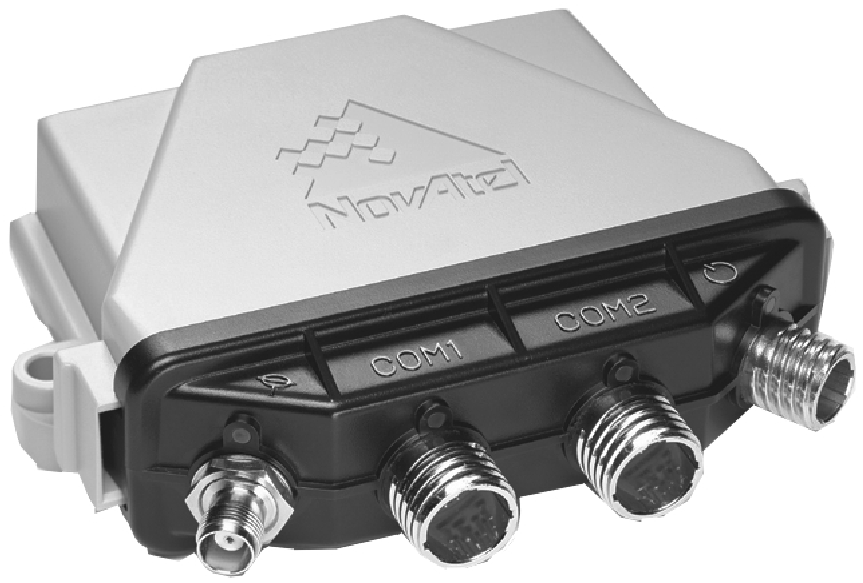
\includegraphics[width=0.4\linewidth]{figures/novatel_flexpak.png}}
	\subcaptionbox{Novatel GPS-701-GG antenna\label{subcap:novatel_antenna}}{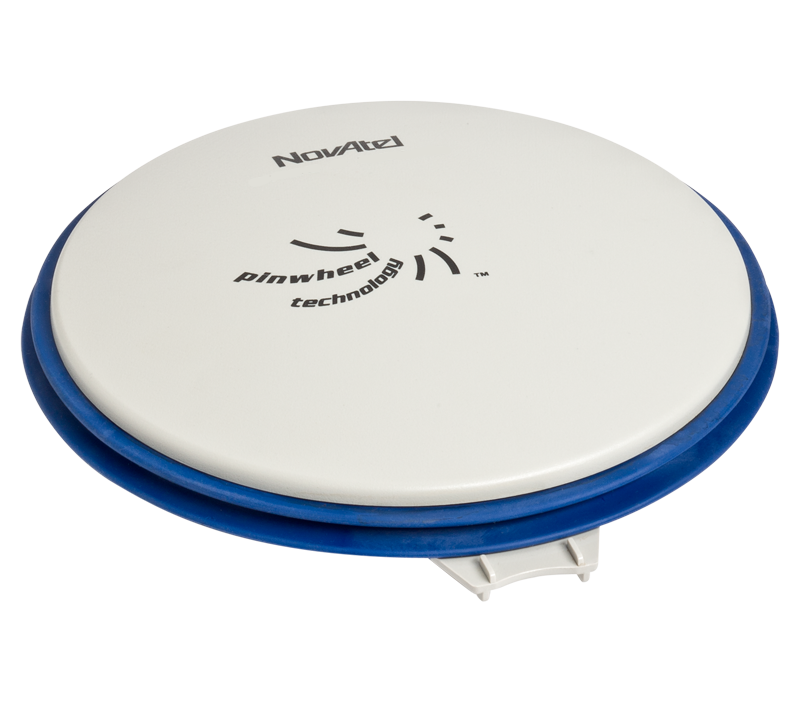
\includegraphics[width=0.4\linewidth]{figures/Novatel_701-GGL.png}}
	\caption[Novatel GNSS devices used]{Novatel GNSS devices used (\href{https://www.novatel.com}{source:NovAtel})}
	\label{fig:novatel_devices}
\end{figure}

Each  Novatel GPS sensor is composed with Novatel OEM4-G2L FlexPak receiver and
Novatel high performance GPS-701-GG antenna. The Novatel OEM4-G2L FlexPak
receiver provides position and velocity estimations using GPS broadcasted
satellites radio signals. It has two communications ports that can be configured
independently. Additional to common GPS protocols, it has support for custom
Novatel protocols (which will be used) providing the best possible estimation
the receiver can do making it as simple as possible from the point of view of
user. The receiver can handle both L1 and L2 signals provided by satellites
\cite{NovAtel2005_volume1}, however, antenna module only can handle L1 frequency
signal (1575.42MHz)\cite{NovAtel2013_antenna}. Power supply to FlexPak enclosure
should range from 6 to 18 volts DC with typical consumption of 5W. Without
differential GPS methods, the Novatel receiver can achieve up to 1.8 meters
precision \gls{CEP} with single point operation. Output logs data rate is up to
20Hz in binary mode and 10Hz in ASCII format.

Since the receivers used are industrial grade, no particular effort is made to modeling any error source or trying to improve the solution given by it. However is important to have minimal knowledge the limitations of those types of receivers. It is trusted that the reported position and velocity information is the best the sensor could possibly estimate.

The developed library interface full documentation is present in the attach appendix \ref{appendix:novatel}, however is advised to use the online version for granting the most recent \href{https://novatel-oem4-python.readthedocs.io/en/latest/}{updated documentation}.

\subsection{GNSS main errors}\label{subsection:GNSS_main_errors}

The main cause of \gls{GNSS} calculations errors are presented in table \ref{tab:gnss_error_source}.
While some can't be controlled by user (satellite clocks, orbit clocks), others can be mitigated using differential GNSS techniques, multi-frequency (currently civilians have access to more than one), satellite based augmentations system and multi-constellation or using modeling the error source. Multipath is probably the most user dependent but in some situations hard to avoid for example in streets surround with high buildings general denoted as urban canyons.


\begin{table}[!htb]
	\centering
	\begin{tabular}{lc}
		\toprule
		\textbf{Source}		& \textbf{Value (up to)}\\
		\midrule
		Satellite clocks	& $\pm2$m\\
		Orbit Errors		& $\pm2.5$m\\
		Inospheric Delays	& $\pm5$m\\
		Tropospheric Delays & $\pm0.5$m\\
		Receiver Noise		& $\pm0.3$m\\
		Multipath			& $\pm1$m\\
		\bottomrule
	\end{tabular}
	\caption[Main source of errors in calculations using GNSS]{Main source of errors in calculations using GNSS \cite{NovatelIntroGNSS}}
	\label{tab:gnss_error_source}
\end{table}
\vfill

%-------------------------------------------------------------------------------
% Razor related stuff
%-------------------------------------------------------------------------------
\section{Sparkfun Razor IMU 9DOF} \label{section:sparkfun}

\begin{figure}[!htb]
	\centering
	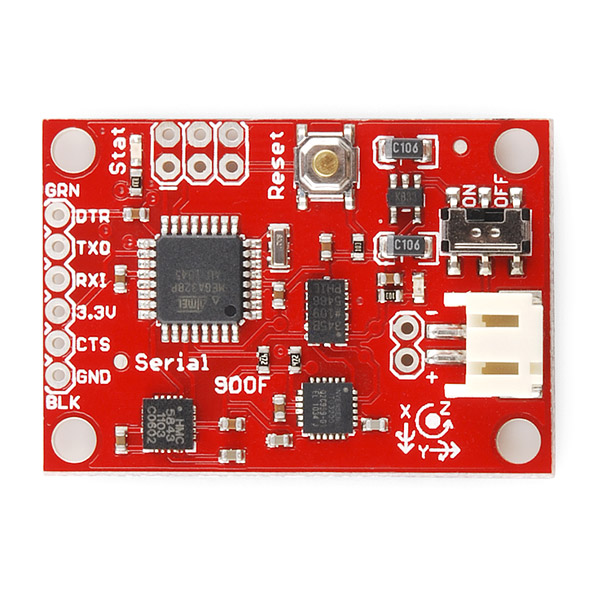
\includegraphics[width=0.5\linewidth]{figures/10125-04b.jpg}
	\caption[Razor 9DOF IMU.]{Razor 9DOF IMU.}
	\label{fig:razor9dof}
\end{figure}

Razor IMU \glsdisp{9DOF}{9DOF} is an electronics board, developed by
\href{http://www.sparkfun.com/}{Sparkfun Electronics}, which includes an
accelerometer, a gyroscope and a magnetometer, each one with three axis of
sensibility. Since this board is based on the
\href{https://www.arduino.cc/}{Arduino project}, the chip sensors are
interconnected by an Atmel\textsuperscript{\textregistered} ATmega328p \gls{MCU}
which allows the configuration of sensors, handles the readings and processing
of their respective outputs. 


%-------------------------------------------------------------------------------
% ADXL345 part
%-------------------------------------------------------------------------------
\subsection{ADXL345 Digital Accelerometer} \label{subsection:adxl345}


The ADXL345 is a \gls{MEMS} sensor with three axis accelerometer made by
\href{http://http://www.analog.com/en/index.html}{Analog Devices} . It has an
adjustable acceleration scale range value up to $\pm16g$. It is possible to
measure both dynamic accelerations resulting from motion and shock or measure
static accelerations such as gravity, which allows this device to be used as a
tilt sensor also. Acceleration deflects the a proof mass attached to one differential capacitor plate and unbalances it, resulting in a sensor output whose amplitude is
proportional to acceleration \cite{adxl345_datasheet}.Conversion of outputs is made through 10 to 13 bit \gls{ADC} according to selected
range to maintain the same scale of 4mg/LSB. 


\subsubsection{Accelerometer sensor model}\label{subsubsection:adxl345model}

The output of accelerometer is proportional to the sum of acceleration in each
axis. However the accelerometer is not capable of distinguish if the
acceleration is caused by a true acceleration produced by motion or produced by
a static force, generally gravity force. As so, equation \eqref{eq:accel_model}
describes the general output of accelerometer \cite{Vectornav_calibration}
where, ${}^bA_{ext}$ is the sum of real external acceleration due to
linear or rotational dynamics in the body frame, ${}^b_wR$ is the rotation
matrix mapping quantities in world frame into sensor frame, ${}^wg $
represents the fictitious acceleration due to gravity in the world frame, ${}^bA_{0}$ is an offset and
$\delta A_{\epsilon}$ describes addictive gaussian noise.
Ideally, $G$ should be equal to identity matrix but in fact it represents the
product of two matrices, one describing the cross-axis influence and the other
a scale factor for each axis \cite{Vectornav_calibration}.

\begin{equation}
{}^bA_{s}=G[{}^bA_{ext} + {}^b_wR\,{}^wg\,] + {}^bA_{0} + \delta A_{\epsilon}
\label{eq:accel_model}
\end{equation}

\subsubsection{Accelerometer calibration}\label{subsubsection:adxl345calibration}

The suggested calibration method by the manufacturer \cite{adxl345AN1077}
assumes that cross-axis influence is small enough and can be neglected, this
way, $G$ should only be represented by a diagonal matrix with the scale factors
for each axis. However, if more precision for the application is needed,
calibration using the ellipsoid fitting approach should be made
\cite{Pylvanainen2008}.

For this application it will be used the suggested calibration by manufacturer
resulting in exposing the sensor to six position combination while resting. This
means the ${}^bA_{ext}$ will be zero and accelerometer will be only
influenced by the gravity force, 1g.

\begin{figure}[!hbt]
	\begin{minipage}{0.49\textwidth}
		\centering
		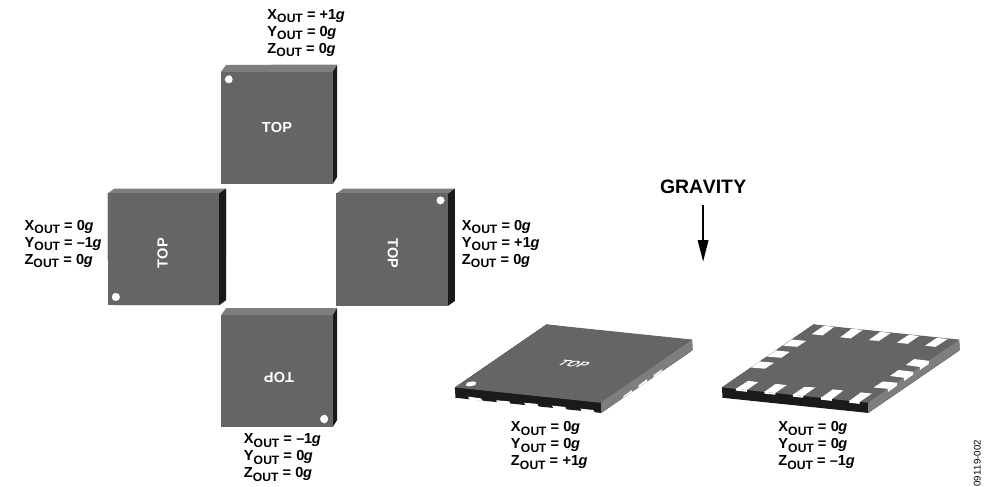
\includegraphics[width=\textwidth]{figures/adxl_calibration.png}
		\caption[ADXL345 calibration poses and expected output.]{ADXL345 calibration
			poses and expected output \cite{adxl345AN1077}.} 
		\label{fig:adxl_calibration}
	\end{minipage}
	\hfill
	\begin{minipage}{0.49\textwidth}
		\renewcommand{\arraystretch}{1.2} % more space between rows
		\centering
		\begin{tabular}{cc}
			\toprule
			\textbf{Gains and offset [LSB]} & \textbf{Razor }\\
			\midrule
			Z gain   &  253.66  \\
			Z offset & -3.47    \\
			Y gain	 & 266.27    \\
			Y offset & -3.18     \\
			X gain   & 266.04   \\
			X offset & 13.83	\\
			\bottomrule
		\end{tabular}
		\captionof{table}{Summary of values extracted and calculated for each axis of accelerometer in both sensors}
		\label{tab:adxl_summary}
	\end{minipage}
\end{figure}

Aligning one axis at a time with gravity vector, as seen in figure
\ref{fig:adxl_calibration}, the mean value of several samples is calculated.
Using these means for each axis and the known acceleration
values(\ensuremath{\pm}1g), it is calculated the slope and offset of the
respective line passing through the two points. Calculated values (see table \ref{tab:adxl_summary}) will be stored
in the internal \glsdisp{EEPROM}{EEPROM} memory of \gls{MCU} to be loaded at
boot time of each razor. The conversion between LSB and g unities is given by
the relation $254LSB/g$ or $3.9mg/LSB$ \cite{adxl345_datasheet}

%-------------------------------------------------------------------------------
% ITG3200 part
%-------------------------------------------------------------------------------
\subsection{ITG3200 Digital Gyroscope} \label{subsection:itg3200}

The ITG-3200 is a microelectronic mechanical integrated circuit chip with three
axis independent gyroscopes, built by
\href{http://www.invensense.com/}{Invensense} able of measuring angular
velocities up to $\pm2000\degree/s$. When the gyroscopes are rotated about any
of the sensor axes, the Coriolis effect causes a deflection that is  detected by
a capacitive pick-off circuit proportional to angular velocity. The measured signal is filtered and converted using internal \gls{ADC}. The scale factor that allow to convert the
output values to angular velocities in degrees per second is, according to its
datasheet \cite{itg3200_datasheet}, factory calibrated and equal to
$14.375LSB/\degree.s^{-1}$.

\subsubsection{Gyroscope sensor model} \label{subsubsection:itg3200model}


For a given axis, the gyroscope output is proportional the angular velocity
sensed of that axis and is given by equation \eqref{eq:gyro_model} where
${}^b\omega_{s}$ represents the vector output of the sensor in body
frame at instant $t$, ${}^b\omega_{real}$ is the real angular velocity
vector applied to sensor in body frame, ${}^b\omega_{0}$ is the bias
vector term and $\delta\omega_{\epsilon}$ addictive gaussian noise.
Since the sensor is described in \cite{itg3200_datasheet} as factory calibrated,
$G$ which represent a scaled factor correction, is expected to be equal to
identity matrix. Note that the equation model \eqref{eq:gyro_model} is in fact a
simplified version of a more accurate model described in
\cite{Vectornav_calibration}. As stated in \cite{Vectornav_calibration}
cross-axis misalignment and linear acceleration sensitivity are expected to be
small for the application purpose so they are considered irrelevant.

In general, the offset value depends on the temperature value inside chip. Once
internal stability is reached, offset values tends to be constant \cite{Woodman2007}. Electrical
temperature stability can be achieved after a few minutes of operation. At the
beginning of initialization of Razor, several samples are acquired internally in
the microprocessor and  mean value is calculated for each axis, defining this
way the offset constant for each axis.


\begin{equation}
{}^b\omega_{s}=G\,{}^b\omega_{real} + {}^b\omega_{0} + \delta\omega_{\epsilon}
\label{eq:gyro_model}
\end{equation}

%-------------------------------------------------------------------------------
% HMC5843 part
%-------------------------------------------------------------------------------
\subsection{HMC5843 Digital compass} \label{subsection:hmc5843} 

The HCM5843 sensor is a digital compass chip designed by
\href{https://www.honeywell.com}{Honeywell}, designed for low field magnetic
sensing. This sensor uses anisotropic magnetic resistor technology, making it
immune to vibration noises, and the use of Wheatstone bridge makes it more
robust to noise. A material with anisotropic magnetic resistor properties
changes its resistance according to absolute value and direction of magnetic
field. 

\subsubsection{Magnetometer model}

The magnetometer sensor model follows a similar structure as two previous
sensors and is given by equation \eqref{eq:mag_model}. The ${}^bH_{s}$ is
the value sensed by the sensor in body frame. $C$ is a matrix resulting from
the multiplication of matrices containing influence of cross-axis, gain scale
factor and soft-iron interference \cite{magAN4246}. ${}^wh_e$ represent
the geomagnetic vector of Earth, ${}^bh_{offset}$ is an offset vector which
describes the influence of zero-field offset and the ferromagnetic masses fixed
relative to body frame usually denoted as hard-iron. $\delta h_{\epsilon}$ 
represents gaussian additive noise.

\begin{equation}
{}^bH_{s}=C\,{}^b_wR{}^wh_e\, + {}^bh_{offset} + \delta h_{\epsilon}
\label{eq:mag_model}
\end{equation}


\subsubsection{Geomagnetic field}\label{subsubsection: geomagnetic_field}

The geomagnetic field can be described as 3D vector in each point as seen in
\cite{ipma_geomagnetism}. As previous defined, ${}^wh_e$ represent the
geomagnetic vector of Earth. Let us define now, ${}^wh_0$ as the
horizontal projection of ${}^wh_e$. The angle between ${}^wh_0$ and
${}^wh_e$ is denominated as inclination, $I$. As stated in
\cite{ipma_geomagnetism}, the horizontal projection of the geomagnetic vector
points to the magnetic north which may not be aligned with the north axis of
reference frame, ${}^wY$. This defines the magnetic declination angle, $D$, as the
angle between horizontal projection and the ${}^wY$ axis.

For Lisbon, the magnetic declination angle, in January 2017, defined in the reference
frame is equal to 2.48\degree, inclination angle is equal to 52.77\degree and
the ${}^wh_e$ is equal to $[-1121.5, 26479.8, -34884.7]^T$ nanoteslas
\cite{noaa}




\subsubsection{Hard and soft-iron compensation}

The compensation for hard and soft-iron effects can be done using a geometric
approach as described by \cite{magAN4246} \cite{Caruso2000}
\cite{Vasconcelos2011}. If the geomagnetic vector is known and sensor perfect
calibrated, free of any type ambient distortion, points collected are expected
to belong a surface of an origin centered sphere with radius equal to the
magnitude of geomagnetic field ${}^wh_e$. Distortions, cross-axis
influence, scale-factor inequalities between axis, causes the expected sphere to
be deformed into a ellipsoid. Collecting points in 3D space by performing
rotations of the sensor frame, allow us to fit the data to an ellipsoid surface
and after determinate the matrix $C$ and offset vector ${}^bh_{offset}$.

However since the body frame is a vehicle, it is not physically possible to
collect points based in rotations of YY and XX axis. Only ZZ axis rotations are
available and the data instead of belonging to an ellipsoid surfaces, will
belong to an ellipse in Z-plane as a result from that plan cutting the ellipsoid
in some undetermined z coordinate. Because of restriction stated before it will
be considered that the influence in ZZ axis is zero and the scale
factor is equal to one. Offset in ZZ axis will also be considered zero. In \cite{thesis_BT} is shown that this assumption is not relevant. \eqref{eq:mag_model} will be rearranged to equation \eqref{eq:mag_model1}
form.

\begin{equation}
\begin{aligned}
{}^bH_{s}&=C\,{}^b_wR{}^wh_e\, + {}^bh_{offset} + \delta h_{\epsilon}\\
{}^b_wR{}^wh_e &=C^{-1}[{}^bH_{s}-{}^bh_{offset} - \delta h_{\epsilon}] \\
\end{aligned}
\label{eq:mag_model1}
\end{equation}

Without loss of generality, $C^{-1}\delta h_{\epsilon}$ will result
also in a gaussian vector so it will be rewritten as $\delta
h_{\epsilon}$. Equation \eqref{eq:mag_model1} can take now be arranged into \eqref{eq:mag_model2} where ${}^bH_{c}$ is the corrected value
after calibration process.

\begin{equation}
\begin{aligned}
{}^b_wR(t){}^wh_e &=C^{-1}[{}^bH_{s}-{}^bh_{offset} - \delta h_{\epsilon}] \\
{}^bH_{c} &= C^{-1}[{}^bH_{s}-{}^bh_{offset}] + \delta h_{\epsilon}
\end{aligned}
\label{eq:mag_model2}
\end{equation}

The matrix $C^{-1}$ and ${}^bh_{offset}$ is obtained as described by
\cite{Caruso2000} using the
\textit{ellipse\_fit}\footnote{\href{https://www.mathworks.com/matlabcentral/fileexchange/22423-ellipse-fit}{https://www.mathworks.com/matlabcentral/fileexchange/22423-ellipse-fit}}. The function \textit{ellipse\_fit} returns the least square estimate that best fits the data collected from sensor and the parameters that define the estimated ellipse as described in \hyperref[list:ellipsfit_out]{this list}:

\begin{itemize}[noitemsep]
	\label{list:ellipsfit_out}  
	\item \textbf{semi-major} - The length of major semi axis of ellipse. 
	\item \textbf{semi-minor} - The length of minor semi axis of ellipse. 
	\item $\bm{x_0}$ - The offset in the XX axis of ellipse.
	\item $\bm{y_0}$ - The offset in the YY axis of ellipse.
	\item $\bm{\alpha}$ - Rotation angle between semi-major axis and XX axis in reference frame.
\end{itemize}

\begin{figure}[!htb]
	\centering
	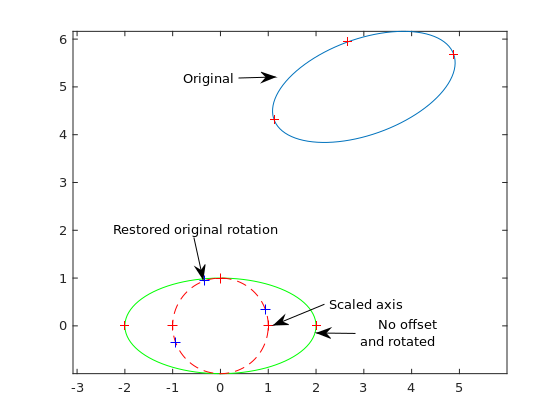
\includegraphics[width=0.7\linewidth]{figures/mag_calibration_steps.png}
	\caption[Calibration steps of ellipse data]{Simulation of the calibration steps applied to hypothetical ellipse data.}
	\label{fig:mag_cal_steps_fig}
\end{figure}

Take note the fact that since is not physically possible to perform rotations in
3D space, the calibration will only be reflect the XX and YY axis. Using the
values returned, the calibration process consists in the following sequential
steps:

\circled{1} Remove offset by using equation \eqref{eq:mag_cal_step1} with ${}^bh_{offset} = [{}^bx_0, {}^by_0, 0]^T$

\begin{equation}
{}^bH_{s}={}^bH_{s}-{}^bh_{offset}
\label{eq:mag_cal_step1}
\end{equation}

\circled{2} Align semi-major axis of ellipse with the XX axis of reference frame using a rotation of $-\alpha$ by using equation \eqref{eq:mag_cal_step2}

\begin{equation}
\begin{aligned}
{}^bH_{s}&=R_{cal}\,{}^bH_{s}\Leftrightarrow\\
\Leftrightarrow{}^bH_{s}&=\begin{bmatrix}
\cos(\alpha) & -\sin(\alpha) & 0\\
\sin(\alpha) & \cos(\alpha)  & 0\\
0			 & 0			 & 1
\end{bmatrix}{}^bH_{s}
\end{aligned}
\label{eq:mag_cal_step2}
\end{equation}

\circled{3} Apply a scaling matrix $S$ to make semi-major axis the same length as semi-minor axis using \eqref{eq:mag_cal_step3}

\begin{equation}
\begin{aligned}
{}^bH_{s}&=S\,{}^bH_{s}\Leftrightarrow\\
\Leftrightarrow{}^bH_{s}&=\begin{bmatrix}
\frac{semi-minor}{semi-major} & 0 & 0\\
0 & 1 & 0\\
0 & 0 & 1
\end{bmatrix}{}^bH_{s}
\end{aligned}
\label{eq:mag_cal_step3}
\end{equation}

\circled{4} Restore the initial rotation $\alpha$ to the scaled data using the transpose of $R_{cal}$ as seen in \eqref{eq:mag_cal_step4}

\begin{equation}
\begin{aligned}
{}^bH_{s}&=R^T_{cal}\,{}^bH_{s}\Leftrightarrow\\
\Leftrightarrow{}^bH_{s}&=\begin{bmatrix}
\cos(\alpha) & \sin(\alpha) & 0\\
-\sin(\alpha) & \cos(\alpha)  & 0\\
0			 & 0			 & 1
\end{bmatrix}{}^bH_{s}
\end{aligned}
\label{eq:mag_cal_step4}
\end{equation}

The ${}^bH_{s}$ resulting from step four is in fact the expected
corrected reading of sensor, ${}^bH_{c}$. In figure
\ref{fig:mag_cal_steps_fig} visually represented the steps applied to a
hypothetical ellipse. Resuming, all sequential steps in one equation results in
\eqref{eq:mag_cal_resume}.

\begin{equation}
{}^bH_{c}=R_{cal}\,S\,R^T_{cal}[{}^bH_{s}-{}^bh_{offset}]
\label{eq:mag_cal_resume}
\end{equation}

Comparing the structure of \eqref{eq:mag_cal_resume} with \eqref{eq:mag_model2} this implies that $C^{-1}$ is equal to $R_{cal}\,S\,R^T_{cal}$. 

The results of calibration are presented for one of the devices in figure
\ref{fig:mag_cal_din0} and the obtained are expressed in the table
\ref{tab:mag_cal_results}. The trajectory used is not important as long as it is
able perform one or more rotation of the vehicle in the horizontal plan. In
figure \ref{subcap:mag_cal_comparison} is shown the results before and after
calibration for the estimation of Euler $\psi$ angle. It is also present the
estimation of the same angle using the the one of the gps unities as a reference
for the comparison.

\begin{figure}[!htp]
	\centering
	\subcaptionbox{Trajectory used for calibration.\label{subcap:mag_cal_din0_gps}}{\includegraphics[width=0.32\linewidth]{Figures/mag_calibration_steps_din0_gps.pdf}}
	\hfill
	\subcaptionbox{Magnetometer calibration \label{subcap:mag_cal_din0}}{\includegraphics[width=0.32\linewidth]{Figures/mag_calibration_steps_din0.pdf}}
	\hfill
	\subcaptionbox{$\psi$ angle estimation before and after calibration of magnetometers\label{subcap:mag_cal_comparison}}{\includegraphics[width=0.32\linewidth]{Figures/mag_calibration_compare.pdf}}
	\caption{Magnetometer calibration steps applied to real data}
	\label{fig:mag_cal_din0}
\end{figure}


\begin{table}[!hbt]
	\centering
	\begin{tabular}{ccc}
		\toprule
		{} & \textbf{Razor 1} \\
		\midrule
		${}^bh_{offset}\quad[nT]$ &[-2.5828\, -2.1703]\textsuperscript{T}x10\textsuperscript{4} \\
		\addlinespace[5pt]
		$\alpha\quad [deg]$ & 107.5238 \\
		\addlinespace[5pt]
		$\frac{semi-minor}{semi-major}$ & 0.9567\\
		\addlinespace[5pt]
		$R_{cal}$ & $\begin{bmatrix}
		-0.3011 & -0.9536 & 0 \\
		+0.9536 & -0.3011 & 0 \\
		0		 &  0	   & 1 \end{bmatrix}$ \\
		\addlinespace[5pt]
		$C^{-1} $ &$\begin{bmatrix}
		+0.9961& +0.0124 & 0\\
		+0.0124& +0.9606 & 0\\
		0     & 0      & 1
		\end{bmatrix} $		 \\
		\addlinespace[5pt]
		\bottomrule
	\end{tabular}
	\caption{Magnetometers calibration results.}
	\label{tab:mag_cal_results}
\end{table}

